% Forked 2026-10-23 from the Earlham PHY 360 (Mathematical Physics) handout
% ~/Library/CloudStorage/Dropbox/__EARLHAM/Courses/360-Mathematical_Physics/ClassHandouts/SimpleNoetherNotes.tex
% (rev. 2023-03-24) for Smith PHY 317 (Classical Mechanics). Changes since the fork: git log.
\documentclass[12pt]{article}
%% Document setup for Syllabus and HW

\textwidth=7in
\textheight=9.5in
\topmargin=-1in
\headheight=0in
\headsep=.5in
\hoffset  -.85in

\usepackage{amsmath} % for \text{}
\usepackage{amsfonts} % For \text{}
\usepackage{amssymb} % For \text{}
\usepackage{amsthm}
\usepackage{bigints}

%% Stolen from Nathan Baker
\newcommand{\erf}{{\mathrm{erf}}}
\newcommand{\erfc}{{\mathrm{erfc}}}
\newcommand{\erfi}{{\mathrm{erfi}}}
\newcommand{\argh}{{\mathrm{arg}}}
\newcommand{\atan}{{\mathrm{atan}}}
\newcommand{\acos}{{\mathrm{acos}}}
\newcommand{\asin}{{\mathrm{asin}}}
\newcommand{\mat}[1]{\,\underline{\underline{#1}}\,}
\newcommand{\abs}[1]{\left| #1 \right|}
\newcommand{\norm}[1]{\left\| #1 \right\|}
\newcommand{\order}[1]{{\mathcal{O}} \left( #1 \right)}
\newcommand{\op}[1]{{\mathcal{#1}}}
\newcommand{\myfile}[1]{\texttt{#1}}
\newcommand{\myvar}[1]{\textsf{#1}}
\newcommand{\mean}[1]{{\left\langle {#1} \right\rangle}}

% The master boolean -- set this to "masterfalse" or "mastertrue"
%\newif\ifmaster \masterfalse
\newif\ifmaster \mastertrue

\newcommand{\hidesolution}[1]{ \ifmaster { {#1} } \else { {Go to class.} } \fi }
\newcommand{\hideanswer}[1]{ \ifmaster { #1 } \else {} \fi }
\newcommand{\solution}[1]{ \begin{proof}[Solution] \hidesolution{#1} \end{proof} }
\newcommand{\answer}[1]{ \hideanswer{\begin{proof}[Answer] #1 \end{proof}} }

%% MGL
\newcommand{\CC}{\mathbb{C}}
\newcommand{\N}{\mathbb{N}}
\newcommand{\Ham}{\mathcal{H}}
%\newcommand{\vect}[1]{\,\vec{\mathbf{#1}}\,}
\newcommand{\vect}[1]{\,\mathbf{#1}\,}
\usepackage{tabularx}
\newcommand{\vtau}{\vect{\tau}}
\newcommand{\vomega}{\vect{\omega}}
\newcommand{\va}{\vect{a}}
\newcommand{\vb}{\vect{b}}
\newcommand{\vc}{\vect{c}}
\newcommand{\vd}{\vect{d}}
\newcommand{\ve}{\vect{e}}
\newcommand{\vf}{\vect{f}}
\newcommand{\vg}{\vect{g}}
\newcommand{\vh}{\vect{h}}
\newcommand{\vi}{\vect{i}}
\newcommand{\vj}{\vect{j}}
\newcommand{\vk}{\vect{k}}
\newcommand{\vl}{\vect{l}}
\newcommand{\vm}{\vect{m}}
\newcommand{\vn}{\vect{n}}
\newcommand{\vo}{\vect{o}}
\newcommand{\vp}{\vect{p}}
\newcommand{\vq}{\vect{q}}
\newcommand{\vr}{\vect{r}}
\newcommand{\vs}{\vect{s}}
\newcommand{\vt}{\vect{t}}
\newcommand{\vu}{\vect{u}}
\newcommand{\vv}{\vect{v}}
\newcommand{\vw}{\vect{w}}
\newcommand{\vx}{\vect{x}}
\newcommand{\vy}{\vect{y}}
\newcommand{\vz}{\vect{z}}

\newcommand{\vA}{\vect{A}}
\newcommand{\vB}{\vect{B}}
\newcommand{\vC}{\vect{C}}
\newcommand{\vD}{\vect{D}}
\newcommand{\vE}{\vect{E}}
\newcommand{\vF}{\vect{F}}
\newcommand{\vG}{\vect{G}}
\newcommand{\vH}{\vect{H}}
\newcommand{\vI}{\vect{I}}
\newcommand{\vJ}{\vect{J}}
\newcommand{\vK}{\vect{K}}
\newcommand{\vL}{\vect{L}}
\newcommand{\vM}{\vect{M}}
\newcommand{\vN}{\vect{N}}
\newcommand{\vO}{\vect{O}}
\newcommand{\vP}{\vect{P}}
\newcommand{\vQ}{\vect{Q}}
\newcommand{\vR}{\vect{R}}
\newcommand{\vS}{\vect{S}}
\newcommand{\vT}{\vect{T}}
\newcommand{\vU}{\vect{U}}
\newcommand{\vV}{\vect{V}}
\newcommand{\vW}{\vect{W}}
\newcommand{\vX}{\vect{X}}
\newcommand{\vY}{\vect{Y}}
\newcommand{\vZ}{\vect{Z}}
%\newcommand{\pd}[2]{\frac{\partial#1}{\partial#2}}
%\newcommand{\dd}[2]{\frac{d#1}{d#2}}
\newcommand{\dinline}[2]{d #1/d #2} % for derivatives
\newcommand{\pdinline}[2]{\partial#1/\partial#2}

\newcommand{\boldcent}[1] {\begin{center}\textbf{ #1 }\end{center}}
% ***********************************************************
% ******************* PHYSICS HEADER ************************
% ***********************************************************
% From http://www.dfcd.net/articles/latex/latex.html
% Version 2
%\documentclass[11pt]{article} 
\usepackage{amsmath} % AMS Math Package
\usepackage{amsthm} % Theorem Formatting
\usepackage{amssymb}	% Math symbols such as \mathbb
\usepackage{graphicx} % Allows for eps images
\usepackage{multicol} % Allows for multiple columns
%\usepackage[dvips,letterpaper,margin=0.75in,bottom=0.5in]{geometry}
% % Sets margins and page size
%\pagestyle{empty} % Removes page numbers
%\makeatletter % Need for anything that contains an @ command 
%\renewcommand{\maketitle} % Redefine maketitle to conserve space
%{ \begingroup \vskip 10pt \begin{center} \large {\bf \@title}
%	\vskip 10pt \large \@author \hskip 20pt \@date \end{center}
%  \vskip 10pt \endgroup \setcounter{footnote}{0} }
%\makeatother % End of region containing @ commands
\renewcommand{\labelenumi}{(\alph{enumi})} % Use letters for enumerate
% \DeclareMathOperator{\Sample}{Sample}
\let\vaccent=\v % rename builtin command \v{} to \vaccent{}
\renewcommand{\v}[1]{\ensuremath{\mathbf{#1}}} % for vectors
\newcommand{\gv}[1]{\ensuremath{\mbox{\boldmath$ #1 $}}} 
% for vectors of Greek letters
\newcommand{\uv}[1]{\ensuremath{\mathbf{\hat{#1}}}} % for unit vector
%\newcommand{\abs}[1]{\left| #1 \right|} % for absolute value
\newcommand{\avg}[1]{\left< #1 \right>} % for average
%\let\underdot=\d % rename builtin command \d{} to \underdot{}
%\renewcommand{\d}[2]{\frac{d #1}{d #2}} % for derivatives
\newcommand{\fd}[2]{\frac{d #1}{d #2}} % for derivatives
\newcommand{\dd}[2]{\frac{d^2 #1}{d #2^2}} % for double derivatives
\newcommand{\pd}[2]{\frac{\partial #1}{\partial #2}} 
% for partial derivatives
\newcommand{\pdd}[2]{\frac{\partial^2 #1}{\partial #2^2}} 
\newcommand{\pddx}[3]{\frac{\partial^2 #1}{\partial #2 \partial #3}} 
% for double partial derivatives
\newcommand{\pdc}[3]{\left( \frac{\partial #1}{\partial #2}
 \right)_{#3}} % for thermodynamic partial derivatives
\newcommand{\ket}[1]{\left| #1 \right>} % for Dirac bras
\newcommand{\bra}[1]{\left< #1 \right|} % for Dirac kets
\newcommand{\braket}[2]{\left< #1 \vphantom{#2} \right|
 \left. #2 \vphantom{#1} \right>} % for Dirac brackets
\newcommand{\matrixel}[3]{\left< #1 \vphantom{#2#3} \right|
 #2 \left| #3 \vphantom{#1#2} \right>} % for Dirac matrix elements
\newcommand{\grad}[1]{\gv{\nabla} #1} % for gradient
\let\divsymb=\div % rename builtin command \div to \divsymb
\renewcommand{\div}[1]{\gv{\nabla} \cdot #1} % for divergence
\newcommand{\tdiv}[1]{\text{div} #1} % for divergence
\newcommand{\curl}[1]{\gv{\nabla} \times #1} % for curl
\newcommand{\lap}[1]{\gv{\nabla}^{2} #1} % for gradient
\let\baraccent=\= % rename builtin command \= to \baraccent
\renewcommand{\=}[1]{\stackrel{#1}{=}} % for putting numbers above =
\newtheorem{prop}{Proposition}
\newtheorem{thm}{Theorem}[section]
\newtheorem{lem}[thm]{Lemma}
\theoremstyle{definition}
\newtheorem{dfn}{Definition}
\theoremstyle{remark}
\newtheorem*{rmk}{Remark}

% ***********************************************************
% ********************** END HEADER *************************
% ***********************************************************


\usepackage[utf8]{inputenc}
\usepackage{xcolor}
\usepackage{pgfplots}
\pgfplotsset{compat=1.18}
% Colors for the shortest-path example (from the 2023 board slide)
\definecolor{etablue}{rgb}{0.0,0.25,0.8}
\definecolor{deadred}{rgb}{0.8,0.0,0.0}
\definecolor{lemmagreen}{rgb}{0.0,0.5,0.15}

% Theorems and definitions
\newtheorem{firstorderinvariant}{First-Order Invariant}
% These are defined so that I can switch to q_i if I think it's clearer.
\newcommand{\muidx}{\mu}
\newcommand{\coord}{x}
\newcommand{\Coord}{X}
\newcommand{\xd}{\dot{\coord}}
\newcommand{\xdd}{\ddot{\coord}}
\newcommand{\Xd}{\dot{\Coord}}
\newcommand{\xmu}{\coord^\mu}
\newcommand{\xnu}{\coord^\nu}
\newcommand{\xmup}{\coord^{\mu{'}}}
\newcommand{\Xmu}{\Coord^\mu}
\newcommand{\Xdmu}{\Xd^\mu}
\newcommand{\xdmu}{\xd^\mu}
\newcommand{\pmu}{p_\mu}
\newcommand{\pdmu}{\dot{p}_\mu}
% \pagestyle{empty}
\numberwithin{equation}{section}

\begin{document}
\title{Highlights from the Noether's Theorem part of our class}
\author{Michael G. Lerner}
\date{\today}

\maketitle


These notes closely follow Dwight Neuenschwander's absolutely lovely book.\cite{neuenschwander2017emmy} They are rearranged, streamlined, and simplified to better fit a small number of lectures.



\setlength{\unitlength}{1in}

\begin{picture}(6,.1) 
\put(0,0) {\line(1,0){6.25}}         
\end{picture}

\section{Background Definitions}

Functionals ($J$) map functions to real numbers. Ours are definite integrals, and we'll call the integrand the Lagrangian, $L$. Our workhorse examples will be the length functional:

\begin{equation}
  \label{eq:lengthJ}
%  J = \left {\int_a^b} \sqrt{1+\left(\fd{y}{x}\right)^2} dx \right. % should work@!!@
  J = \bigintss_a^b \sqrt{1+\left(\fd{y}{x}\right)^2} dx
\end{equation}

and the action functional:

\begin{equation}
  \label{eq:action}
  J = \int_a^b (K-U) dt
\end{equation}

We always  call the integrand of the functional ``the Lagrangian,''
denoted $L$. This is slightly nonstandard terminology, but we want to
have a single word for the integrand of the functional that includes
length as well as the standard $K-U$. For the rest of this handout,
unless otherwise specified, you may assume that general equations and
theorems are referring to the following functional:

Let $J$ be a functional whose Lagrangian depends on one independent
variable $t$, $N$ dependent variables $\xmu(t)$, and their $N$
derivatives $\xdmu$, $\muidx=1,2,...,N$:

\begin{equation}
  \label{eq:fmain}
  J = \int_a^b L(t,\xmu,\xdmu)dt
\end{equation}

We will often need to consider functions that are first-order invariant.

\begin{firstorderinvariant}
We will call a function $F(\epsilon)$ first-order invariant in $\epsilon$ if its power series expansion has $a_1=0$:

\begin{equation}
  \label{eq:firstorderinvariant}
  \begin{matrix}
    F(\epsilon) &=& a_0 &+& a_1\epsilon &+& a_2\epsilon^2 &+&...& \\ 
                &=& a_0 & &             &+& a_2\epsilon^2 &+&...& \quad .
 \end{matrix}
\end{equation}

The main reason we'll want this particular condition becomes clear
when you look at  $(\dinline{F}{\epsilon})_{\epsilon=0}$, also written $F'(0)$, i.e. $\dinline{F}{\epsilon}$ evaluated at
$\epsilon=0$. First-order invariance is exactly the condition we need
for this quantity to be zero.

\end{firstorderinvariant}

\section{Examples}

Before we move on to the heavy lifting of proofs, let's talk about
where we're going. First, we're going to start with classical
mechanics, where this useful thing called the Lagrangian is defined as
$L\equiv K-U$, the difference between the kinetic and potential energy
of a system. If we write that out for a one-dimensional, one-particle
system (here, we'll use a pool ball on a horizontal pool table), we get

\begin{eqnarray}
  \textrm{Kinetic:} & K &= \frac{1}{2}m\xd^2 \\
  \textrm{Potential:} & U &= mgh\\
  \label{eq:poolL}
  \textrm{Lagrangian:} & L &= \frac{1}{2}m\xd^2 - mgh
\end{eqnarray}

It turns out (\S\ref{sec:n2l-ham}) that the ``action,'' i.e. the
definite integral of that thing, is pretty important. We'll be able to
say two things about it pretty quickly. First, let's see what happens
to it under a translation in space. We'll define that to be

\begin{equation}
  \coord \to \coord' = \coord + \epsilon
\end{equation}

which gives us a nice one-parameter family of translations (change
$\epsilon$, get a new translation). We want to say that $J$ is
invariant under that translation. This will be the first half of our
``invariant + extremal = conserved quantity.'' 

\begin{eqnarray}
  J & =& \int_a^b L(t,\xmu,\xdmu)dt\\
    & =&  \int_a^b \left(\frac{1}{2}m\xd^2 - mgh \right)dt
\end{eqnarray}

Under our coordinate transformation, we replace each instance of
$\coord$ with $\coord + \epsilon$. Since $\coord$ doesn't actually
appear at all in our functional, we can pretty clearly conclude that
the functional is invariant under the transformation. We could just as
easily write that last sentence as

\begin{equation}
  \label{eq:introalmost}
  0 = \left(\pd{L}{\epsilon}\right)_{\epsilon=0} = \textrm{something.}
\end{equation}

The second key to Noether's theorem is ``extremal.'' We'll find out
that, when functionals are extremal, we can use the Euler-Lagrange
equations. Applying the Euler-Lagrange equations to the ``something''
in \eqref{eq:introalmost} tells us that 

\begin{equation}
  0 = \fd{}{t}\left(\pd{L}{\xd}\right)
\end{equation}

\noindent i.e. that $\pd{L}{\xd}$ is conserved. Well that's
convenient! If we look at \eqref{eq:poolL}, we see that taking that
derivative gives us $m\xd$, or the momentum. Ta-da! We've shown that
an invariant (our translation in space) plus the fact that $J$ had to
be extremal gave us a conservation law!

Similarly, we'll find that a translational symmetry in time ($t \to t'
= t + \epsilon$) will give us conservation of energy!

\section{When are functionals extremal, part 1}
\subsection{Simple Euler-Lagrange}
\label{sec:simple-el}

We want to find the $y(x)$ which will make

\begin{equation}
  J = \int_{x_1}^{x_2}F(x,y,y')dx
\end{equation}

an extremal (also called stationary). Consider the set of varied curves

\begin{equation}
  Y(x) = y(x) + \epsilon\eta(x), \qquad \eta(x_1) = \eta(x_2) = 0
\end{equation}

for one specific $\eta$ with the given boundary conditions. That is, we are considering a continuous single-parameter family of curves for which $\epsilon=0$ gives us $y(x)$. Then we have $J$ as a function of $\epsilon$, and we can write this in several ways:

\begin{equation}
  J = J(\epsilon) = \int_{x_1}^{x_2}F(x,Y,Y')dx = J(\epsilon,y,y',\eta)
\end{equation}

further, we know that we want to make $J$ an extremum (for example, a minimum) when $\epsilon=0$ (that's another way of saying we want $y$ to be extremal). I.e., we want

\begin{equation*}
  \fd{J}{\epsilon}=0 \qquad\textrm{when}\quad\epsilon=0
\end{equation*}
or
\begin{equation}
  \label{eq:djde0}
  \left( \fd{J}{\epsilon}\right)_{\epsilon=0} = 0
\end{equation}

We write out $\fd{J}{\epsilon}$ via the chain rule:

\begin{equation}
  \label{eq:djdechain}
  \fd{J}{\epsilon} = \int_{x_1}^{x_2}\left(\pd{F}{Y}\pd{Y}{\epsilon} + \pd{F}{Y'}\pd{Y'}{\epsilon}\right) dx
 = \int_{x_1}^{x_2}\left(\pd{F}{Y}\eta(x) + \pd{F}{Y'}\eta'(x)\right) dx
\end{equation}

Now, we want \ref{eq:djde0}, so we set $\epsilon=0$ to turn the $Y$'s into $y$'s and get

\begin{equation}
  \left( \fd{J}{\epsilon}\right)_{\epsilon=0} =  \int_{x_1}^{x_2}\left(\pd{F}{y}\eta(x) + \pd{F}{y'}\eta'(x)\right) dx = 0
\end{equation}

Integrating the second term by parts gave us

\begin{equation}
  \left( \fd{J}{\epsilon}\right)_{\epsilon=0} =  \int_{x_1}^{x_2} \left( \pd{F}{y} - \fd{}{x}\pd{F}{y'} \right)\eta(x)dx + 
  \left[ \pd{F}{y'}\eta(x)\right]_{x_1}^{x_2}
\end{equation}

Our boundary conditions $\eta(x_1) = \eta(x_2) = 0$ make the bracketed term zero.

It is at this point that we start to think about $\eta$. If our path
$y$ is an extremal, then \ref{eq:djde0} must be true for {\it any}
twice-differentiable $\eta$ satisfying the boundary conditions, as any
such family of curves gives $y$ for $\epsilon=0$. That being the case,
we can apply the Fundamental Lemma (\S\ref{sec:fundlemma}) to the remaining integral. It tells us
that the term in parentheses must be zero, yielding

\begin{equation}
  \label{eq:simple-el}
  \fd{}{x}\pd{F}{y'} = \pd{F}{y}.
\end{equation}

The proof for the multidimensional case was exactly the same, except that we had to add indices to keep track of each dimension. When we used the summation convention, even the chain rule in \ref{eq:djdechain} looked identical.


Wait, what fundamental lemma?

\subsection{The Fundamental Lemma of the Calculus of Variations}
\label{sec:fundlemma}


If $A(t)$ is continuous on the interval $[a,b]$, and
\begin{equation*}
  \int_a^b A(t)\eta(t)dt=0
\end{equation*}
for {\it every} twice-differentiable $\eta(t)$ with $\eta(a)=\eta(b)=0$,
then it must be the case that $A(t) \equiv 0 \quad \forall t \in [a,b]$. To
be clear, the lemma doesn't say ``the only way the integral of the
product of two functions can be zero is if one is identically zero.''
Rather, it says ``if we are given that this thing is true for
{\it all} $\eta$ satisfying these conditions, then it must be true that $A
\equiv 0$.''

We'll use a proof by contradiction, constructing a ``bad'' function that
met the conditions and was positive in a neighborhood in which $A$
was positive. I got this from Neuenschwander, who mentions that he got
it from Logan 1977. Here goes:

``Proof by contradiction'' may be a bit rusty for some of you. The
strategy is as follows: the above claim is ``if some collection of
conditions is true, then $A(t)$ must be zero everywhere between $a$ and
$b$.'' We'll pretend that the lemma isn't true, i.e. that $A(t)$ can
be nonzero somewhere in that range. We'll find that, much to our
surprise, it leads to a contradiction: no matter what we do, letting
$A(t)$ be nonzero in $[a,b]$ means we {\it cannot} have the
integral equal to zero for every $\eta$. We'll conclude, then, that the only way to
satisfy our collection of conditions (i.e. have the integral equal to
zero) is for $A(t)$ to be zero in $[a,b]$.

Let's do it. First, let's assume that there is some point $c$ between
$a$ and $b$ where $A(c) \neq 0$. Without loss of generality, let's
assume $A(c) > 0$ (if $c$ is an endpoint, continuity hands us a point strictly inside $(a,b)$ where $A$ is still nonzero, so use that one instead; you can rewrite the proof yourself for $A(c) < 0$;
it looks exactly the same but with a few signs switched).

Now, since $A(t)$ is continuous, there must be some neighborhood
around $c$ for which $A$ is positive. We'll call this interval
$(t_1,t_2)$, chosen small enough to sit inside $[a,b]$. All we want to do now is to construct an appropriate $\eta$
to get a contradiction. Geometrically, it's easy to see what we want:
we have an $A(t)$ that has a little positive bump. If we could make an
$\eta$ that was positive in the same region, but zero everywhere else,
the integral of the product would have to be positive.

Having said that, it's straightforward enough. We want $\eta$ to be
zero at $t_1$ and $t_2$, so we'll want something like $(t - t_1)(t - t_2)$
that zeros out at $t_1$ and $t_2$. 

Two little tweaks: first, if $t_1 < t < t_2$, the function we just
picked has something positive times something negative, so it's
overall negative. We wanted $\eta$ to be positive. So, try $(t -
t_1)(t_2 - t)$. So far, so good. Now, we want $\eta(t)$ to have
continuous second derivatives throughout the region $[a,b]$, so let's
make

\[ \eta(t) = \left\{ \begin{array}{ll}
         (t-t_1)^3(t_2-t)^3 & \mbox{if $t_1 < t < t_2$};\\
        0 & \mbox{otherwise}.\end{array} \right. \] 

Well, that does exactly what we wanted: the integral now has to
be positive, but that's the contradiction we were looking for: any
time you choose an $A$ that isn't identically zero, I can make an
$\eta$ that leads to a contradiction. Conclusion: given the stated
conditions, $A(t) \equiv 0$.

\subsection{Example: the shortest path between two points}
\label{sec:shortest-path}

Let's put the last two sections to work on a question where we
already know the answer: what is the shortest path between two points
$(x_1,y_1)$ and $(x_2,y_2)$ in the plane? Everyone ``knows'' it's a
straight line, which makes it a nice test of the machinery. Our goal
is to find the $y(x)$ that makes the length functional
\eqref{eq:lengthJ}
\begin{equation}
  \label{eq:shortJ}
  J = \int_{x_1}^{x_2}\sqrt{1+y'^2}\,dx
\end{equation}
as small as possible, with $y(x_1)=y_1$ and $y(x_2)=y_2$ pinned down.
We could simply plug $F=\sqrt{1+y'^2}$ into \eqref{eq:simple-el}, but
it's worth walking through the argument of \S\ref{sec:simple-el} once
with a specific $F$ in hand, since every step is something you can
draw. In the figures, the curves we get to choose are
\textcolor{etablue}{blue}, the term that dies is
\textcolor{deadred}{red}, and the Fundamental Lemma and what it hands
us are \textcolor{lemmagreen}{green}.

\begin{figure}[!htb]
  \centering
  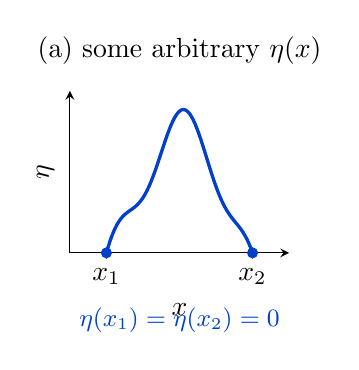
\begin{tikzpicture}[baseline=(ax0.south west)]
    \begin{axis}[name=ax0, width=0.36\textwidth, height=0.3\textwidth,
      axis lines=left, xmin=0, xmax=6, ymin=0, ymax=1.8,
      xtick={1,5}, xticklabels={$x_1$,$x_2$}, ytick=\empty,
      xlabel={$x$}, ylabel={$\eta$}, clip=false,
      title={(a) some arbitrary $\eta(x)$}]
      \addplot[etablue, very thick, domain=1:5, samples=80]
        {(x-1)*(5-x)*(0.3+0.1*sin(deg(2.5*x)))};
      \fill[etablue] (axis cs:1,0) circle (2pt) (axis cs:5,0) circle (2pt);
      \node[etablue, font=\small, align=center] at (axis cs:3,-0.75)
        {$\eta(x_1)=\eta(x_2)=0$};
    \end{axis}
  \end{tikzpicture}\hfill
  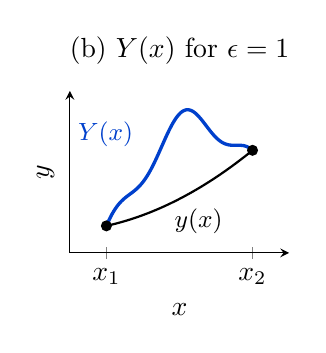
\begin{tikzpicture}[baseline=(ax1.south west)]
    \begin{axis}[name=ax1, width=0.36\textwidth, height=0.3\textwidth,
      axis lines=left, xmin=0, xmax=6, ymin=0, ymax=3,
      xtick={1,5}, xticklabels={$x_1$,$x_2$}, ytick=\empty,
      xlabel={$x$}, ylabel={$y$}, clip=false,
      title={(b) $Y(x)$ for $\epsilon=1$}]
      \addplot[black, thick, domain=1:5, samples=60]
        {0.5+0.15*(x-1)+0.05*(x-1)^2};
      \addplot[etablue, very thick, domain=1:5, samples=80]
        {0.5+0.15*(x-1)+0.05*(x-1)^2 + (x-1)*(5-x)*(0.3+0.1*sin(deg(2.5*x)))};
      \fill (axis cs:1,0.5) circle (2pt) (axis cs:5,1.9) circle (2pt);
      \node[font=\small, below right] at (axis cs:2.6,1.0) {$y(x)$};
      \node[etablue, font=\small, left] at (axis cs:2.0,2.2) {$Y(x)$};
    \end{axis}
  \end{tikzpicture}\hfill
  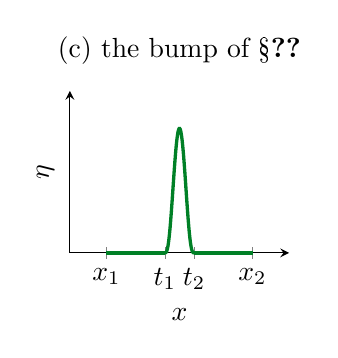
\begin{tikzpicture}[baseline=(ax2.south west)]
    \begin{axis}[name=ax2, width=0.36\textwidth, height=0.3\textwidth,
      axis lines=left, xmin=0, xmax=6, ymin=0, ymax=1.3,
      xtick={1,2.6,3.4,5}, xticklabels={$x_1$,$t_1$,$t_2$,$x_2$},
      ytick=\empty, xlabel={$x$}, ylabel={$\eta$}, clip=false,
      title={(c) the bump of \S\ref{sec:fundlemma}}]
      \addplot[lemmagreen, very thick, domain=1:2.6] {0};
      \addplot[lemmagreen, very thick, domain=2.6:3.4, samples=60]
        {(x-2.6)^3*(3.4-x)^3/0.004096};
      \addplot[lemmagreen, very thick, domain=3.4:5] {0};
    \end{axis}
  \end{tikzpicture}
  \caption{The pictures behind \S\ref{sec:shortest-path}. (a) Any
    curve $\eta$ that vanishes at both ends. (b) The varied curve
    $Y=y+\epsilon\eta$ for $\epsilon=1$; it starts and ends where $y$
    does. (c) The bump $\eta=(x-t_1)^3(t_2-x)^3$ inside $(t_1,t_2)$,
    zero outside, from the proof of the Fundamental Lemma.}
  \label{fig:shortest-path}
\end{figure}

First, we pick some arbitrary curve \textcolor{etablue}{$\eta(x)$}
that vanishes at both ends, \textcolor{etablue}{$\eta(x_1) =
  \eta(x_2) = 0$} (Fig.~\ref{fig:shortest-path}a), and build the
family of varied curves
\begin{equation}
  Y(x) = y(x) + \epsilon\eta(x).
\end{equation}
Because $\eta$ vanishes at the ends, every $Y$ starts and ends at the
same two points as $y$ (Fig.~\ref{fig:shortest-path}b), so every $Y$
is a fair competitor. The length of a varied curve is
\begin{equation}
  J(\epsilon) = \int_{x_1}^{x_2}\sqrt{1+Y'^2}\,dx,
  \qquad Y'(x) = y'(x) + \epsilon\eta'(x),
  \qquad\textrm{so}\qquad \pd{Y'}{\epsilon} = \eta'(x).
\end{equation}
If $y$ is our extremal, then $J(\epsilon)$ is stationary at $\epsilon=0$
(for a shortest path, that's where it bottoms out), so $\dinline{J}{\epsilon}=0$ when $\epsilon=0$. The
limits don't depend on $\epsilon$, so we can differentiate under the
integral sign:
\begin{equation}
  \fd{J}{\epsilon}
  = \int_{x_1}^{x_2}\frac{1}{2}\,\frac{1}{\sqrt{1+Y'^2}}\,2Y'\pd{Y'}{\epsilon}\,dx
  = \int_{x_1}^{x_2}\frac{Y'\eta'}{\sqrt{1+Y'^2}}\,dx .
\end{equation}
Setting $\epsilon=0$ turns the $Y$'s into $y$'s:
\begin{equation}
  \label{eq:short-de}
  \left(\fd{J}{\epsilon}\right)_{\epsilon=0}
  = \int_{x_1}^{x_2}\frac{y'(x)\,\eta'(x)}{\sqrt{1+y'^2}}\,dx = 0 .
\end{equation}
This is the same spot we were in in \S\ref{sec:simple-el} just before
integrating by parts: we know
something about $\eta'$, but the Fundamental Lemma wants $\eta$. So we
integrate by parts with
\begin{equation*}
  u = \frac{y'}{\sqrt{1+y'^2}}, \qquad dv = \eta'(x)\,dx,
  \qquad\textrm{so}\qquad
  du = \fd{}{x}\left(\frac{y'}{\sqrt{1+y'^2}}\right)dx, \qquad v = \eta(x),
\end{equation*}
which gives
\begin{equation}
  0 = \left(\fd{J}{\epsilon}\right)_{\epsilon=0}
  = \underbrace{\textcolor{deadred}{\left[\frac{y'\,\eta(x)}{\sqrt{1+y'^2}}\right]_{x_1}^{x_2}}}_{\textcolor{deadred}{=\,0\textrm{ since }\eta(x_1)=\eta(x_2)=0}}
  - \int_{x_1}^{x_2}\eta(x)\,\fd{}{x}\left(\frac{y'}{\sqrt{1+y'^2}}\right)dx .
\end{equation}
The boundary term dies for exactly the reason we insisted on
$\eta(x_1)=\eta(x_2)=0$. What's left is
\begin{equation}
  \int_{x_1}^{x_2}\eta(x)\,\fd{}{x}\left(\frac{y'}{\sqrt{1+y'^2}}\right)dx = 0
\end{equation}
for \emph{every} $\eta$ that vanishes at the ends. That is precisely
the hypothesis of the \textcolor{lemmagreen}{Fundamental Lemma}
(\S\ref{sec:fundlemma}), with
$A(x) = \dinline{}{x}\bigl(y'/\sqrt{1+y'^2}\bigr)$. To see it in
pictures: if $A$ were positive somewhere, we would park the
\textcolor{lemmagreen}{bump} of Fig.~\ref{fig:shortest-path}c right
there, and the integral would come out positive instead of zero. So
\begin{equation}
  \textcolor{lemmagreen}{\fd{}{x}\left(\frac{y'}{\sqrt{1+y'^2}}\right) = 0
  \quad\Rightarrow\quad \frac{y'}{\sqrt{1+y'^2}} = C}
\end{equation}
for some constant $C$. Squaring and solving, $y'^2 = C^2/(1-C^2)$
(note $|C|<1$ automatically, since $|y'| < \sqrt{1+y'^2}$), and $y'$
has the same sign as $C$, so
\begin{equation}
  \textcolor{lemmagreen}{y' = \frac{C}{\sqrt{1-C^2}} = \textrm{const}
  \quad\Rightarrow\quad y = mx + b,}
\end{equation}
\textcolor{lemmagreen}{a straight line}, with $m$ and $b$ fixed by
making it pass through our two points. Plugging $F=\sqrt{1+y'^2}$
into \eqref{eq:simple-el} gets us here in one line, since
$\pdinline{F}{y}=0$ and $\pdinline{F}{y'} = y'/\sqrt{1+y'^2}$, which
is a nice check.

Two honest caveats. First, $(\dinline{J}{\epsilon})_{\epsilon=0}=0$
tells us the straight line is the only \emph{extremal}; that it is a
minimum (rather than a maximum or something in between) we are happy
to take from geometry here. Second, writing the path as $y(x)$ only
lets us compare curves that never double back in $x$; that's no loss
for the shortest path, but it's an assumption we made.

And now we can prove a version of Noether's Theorem!

\subsection{Invariance}

\subsection{Simple Noether's Theorem}
\label{sec:simplenoether}

The heart of Noether's theorem is that an invariance combined with an
extremal leads to a conserved quantity.

Let our Lagrangian itself (for comparison, see definitions
\ref{eq:inv1} through \ref{eq:inv4}) be first-order invariant in
$\epsilon$ under the change of coordinates

\begin{equation}
  \xmu \to \xmu + \epsilon\Xmu(\coord) 
\end{equation}

where each $\Xmu$ may be a function of all the $\{\xmu\}$ (e.g. we
could send $x \to x + \epsilon(2x+y)$).

Since $L$ is invariant,

\begin{eqnarray}
  0 = \left( \fd{L}{\epsilon}\right)_{\epsilon=0} 
  &=& \sum_\mu{\left( \pd{L}{\xmu}\pd{\xmu}{\epsilon} +  \pd{L}{\xdmu}\pd{\xdmu}{\epsilon} \right)_{\epsilon=0}} \\
  &=&\sum_\mu{\left( \pd{L}{\xmu}\Xmu +  \pd{L}{\xdmu}\Xdmu \right)}.\notag
\end{eqnarray}

That takes care of invariance. Since we want $\xmu$ to be extremal, we
can now use the Euler-Lagrange equation on the first term:

\begin{equation}
0 = \sum_\mu{\left( \fd{}{t}\left(\pd{L}{\xdmu}\right)\Xmu +  \pd{L}{\xdmu}\Xdmu \right)}.
\end{equation}

Using the product rule and pulling the time derivative out of the sum,
we get

\begin{equation}
  0 = \fd{}{t}\left( \sum_\mu{\pd{L}{\xdmu}\Xmu} \right)
\end{equation}

which is our big punchline. We define a ``Noether momentum'' (noting
that it doesn't have to have the units of momentum) to be

\begin{equation}
  P(\xmu,\xdmu) = \sum_\mu{\pd{L}{\xdmu}\Xmu}
\end{equation}

and note that it's conserved, i.e. it doesn't change with time!



\subsection{The Euler-Lagrange Equations}
Let $J$ be as in Eq. \ref{eq:fmain}. Then the $\{\xmu(t)\}$ that make $J$ an
extremal are the solutions of the $N$ Euler-Lagrange equations

\begin{equation*}
  \pd{L}{\xmu} = \fd{}{t}\pd{L}{\xdmu}
\end{equation*}

We gave two proofs of the Euler-Lagrange equations, but they
both boiled down to an integration by parts and an application of the
fundamental lemma. One is included in section \ref{sec:simple-el}.

{\bf In fact, this was enough for us to prove version 1 of Noether's theorem! The proof is reproduced in section \ref{sec:simplenoether}.}

We then defined our conjugate momenta and our Hamiltonian as

\begin{eqnarray*}
  \pmu &\equiv& \pd{L}{\xdmu} \\
  H &\equiv& H(t,\xmu,\pmu) \equiv \pmu\xdmu - L,
\end{eqnarray*}

[side note: we will almost always find that $H$ is the energy. Write $H$ out explicitly for a 1D particle. Does it reduce to the energy?]

which led us to the two canonical ways of writing the Euler-Lagrange
equations. Following Neuenschwander, we'll call them ELE I and ELE II:

\begin{eqnarray}
  \label{eq:ele1}
  \textrm{ELE I:} & \pd{L}{t} &= -\dot{H} = -\fd{}{t} \left[  \xdmu\pd{L}{\xdmu} - L\right ] \\
  \label{eq:ele2}
  \textrm{ELE II:} & \pd{L}{\xmu} &= \pdmu = \fd{}{t}\pd{L}{\xdmu}.
\end{eqnarray}

We also got two conservation laws (conservation of linear momentum and conservation of energy) directly from ELE II and ELE I.

\subsection{Why do we care if functionals are extremal?}
We've mentioned the importance of tasks like finding geodesics, the brachistochrone problem, etc. The most central application to physics, however, is Hamilton's principle, which says that the path a particle takes from point $a$ to $b$ will be the one that minimizes (more precisely, makes stationary) the action as defined in \ref{eq:action}. Section \ref{sec:n2l-ham} shows how Hamilton's principle is a restatement of Newton's second law.

\pagebreak
\section{More Examples}
So far, it seems like we have everything we could need from ELE I and
ELE II. I'm about to tell you to dive into a fancier version of
invariance, called the Rund-Trautman identity. Why should you spend
the time? Here's a great example:

Let's say we want to study a damped simple harmonic oscillator
(SHO). In this case, we would expect that neither momentum nor energy
would be conserved (that's the whole point of damping). Shockingly, a
more advanced version of Noether's theorem will give us a conserved
quantity! First, we'll need to write out our ``Lagrangian'' and the
claim from class was that

\begin{equation}
  L = \left[\frac{1}{2}m\xd^2 - \frac{1}{2}k\coord^2\right]e^{bt/m}
\end{equation}

\noindent which seemed a little odd to us. What I'd forgotten in my
excitement is that Neuenschwander is a little unique in his
terminology, and sometimes it causes me to slip up. The Lagrangian in
this world is not strictly ``$L=K-U$;'' rather, it's ``the integrand
of the functional.'' Fair enough. 

In classical mechanics, one typically takes the Lagrangian, plugs it
into the Euler-Lagrange equations, and obtains the equation of motion
for a particle.  If we have an undamped SHO, we could just write
Newton's second law to get the equation of motion directly:

\begin{equation}
  F = -k\coord = m\xdd
\end{equation}

If we assume a linear restoring and damping force with damping
constant $b$, Newton's second law turns into

\begin{equation}
  -k\coord - b\xd = m \xdd
\end{equation}

\noindent (the ``linear'' in ``linear damping force'' means that we
depend linearly on the velocity, $\xd$). So, our question at hand is,
what ``Lagrangian'' would give us that equation of motion?

\section{Invariance}

Under the transformation

\begin{eqnarray}
  t \to t' = & T(t,q^\mu,\epsilon) = & t + \epsilon\tau + ..., \qquad \tau(t,q^\mu)=\left(\fd{T}{\epsilon}\right)_0\\
  q^\mu \to q^{\mu{'}} = & Q^\mu(t,q^\mu,\epsilon) = & q^\mu + \epsilon\zeta^\mu + ...,  \qquad \zeta^\mu(t,q^\nu)=\left(\fd{Q^\mu}{\epsilon}\right)_0\notag
\end{eqnarray}

Definition 1: 

\begin{equation}
  \label{eq:inv1}
  J-J'=0
\end{equation}

Definition 2: 

\begin{equation}
  \label{eq:inv2}
  J-J' \sim \epsilon^{s}, \qquad s>1
\end{equation}

Definition 3:

\begin{equation}
  \label{eq:inv3}
  L'\fd{t'}{t} - L \sim \epsilon^s , \qquad s>1
\end{equation}

Definition 4: a functional is {\it divergence invariant} if, for some
function $F(t)$,

\begin{equation}
  \label{eq:inv4}
  L'\fd{t'}{t} - L  = \epsilon \fd{F}{t} + O(\epsilon^s) , \qquad s>1
\end{equation}

Explicit verification of these things is quite involved, and our life
is made much easier by application of the Rund-Trautman identity:

Iff $J$ is invariant under \ref{eq:inv3}, the following identity holds:

\begin{equation}
  \label{eq:rti1}
  \textrm{RTI I:}\qquad\pd{L}{q^\mu}\zeta^\mu + p_\mu\dot{\zeta}^\mu + \pd{L}{t}\tau - H\dot{\tau} = 0
\end{equation}

We can use the product rule to get 

\begin{equation}
  \label{eq:rti2}
  \textrm{RTI II:}\qquad-\left( \zeta^\mu - \dot{q}^\mu\tau \right)\left[ \pd{L}{q^\mu} - \fd{}{t}\pd{L}{\dot{q}^\mu}  \right]
    = \fd{}{t}\left[ p_\mu\zeta^\mu - H\tau  \right]
\end{equation}

Iff $J$ is divergence invariant under \ref{eq:inv4}, the following identity holds:

\begin{equation}
  \label{eq:rti1inhom}
  \textrm{RTI I:}\qquad\pd{L}{q^\mu}\zeta^\mu + p_\mu\dot{\zeta}^\mu + \pd{L}{t}\tau - H\dot{\tau} = \fd{F}{t}
\end{equation}

We can use the product rule to get 

\begin{equation}
  \label{eq:rti2inhom}
  \textrm{RTI II:}\qquad-\left( \zeta^\mu - \dot{q}^\mu\tau \right)\left[ \pd{L}{q^\mu} - \fd{}{t}\pd{L}{\dot{q}^\mu}  \right]
    = \fd{}{t}\left[ p_\mu\zeta^\mu - H\tau  - F\right]
\end{equation}

\section{Extremal + Invariance = Noether's Theorem}

If the functional

\begin{equation*}
  J = \int_a^b L(t,\xmu,\xdmu)dt
\end{equation*}

is an extremal, and if under the infinitesimal transformation

\begin{eqnarray*}
  t \to t' = & T(t,\xmu,\epsilon) = & t + \epsilon\tau + ..., \qquad \tau(t,\xmu)=\left(\fd{T}{\epsilon}\right)_0\\
  \xmu \to \xmup = & \Xmu(t,\xmu,\epsilon) = & \xmu + \epsilon\zeta^\mu + ...,  \qquad \zeta^\mu(t,\xnu)=\left(\fd{\Xmu}{\epsilon}\right)_0\notag
\end{eqnarray*}

it is divergence invariant according to the inhomogeneous definition

\begin{equation*}
  L'\fd{t'}{t} - L  = \epsilon \fd{F}{t} + O(\epsilon^s) , \qquad s>1
\end{equation*}

then the following conservation law holds:

\begin{equation}
  p_\mu\zeta^\mu - H\tau - F = \textrm{const}.
\end{equation}

where

\begin{eqnarray*}
  \pmu &\equiv& \pd{L}{\xdmu} \\
  H &\equiv& H(t,\xmu,\pmu) \equiv \pmu\xdmu - L,
\end{eqnarray*}


Proof: we have already done all of the heavy lifting. This works with
either form of the Rund-Trautman identity, but is most straightforward with \ref{eq:rti2inhom}:

\begin{equation}
  -\left( \zeta^\mu - \xdmu\tau \right)\left[ \pd{L}{\xmu} - \fd{}{t}\pd{L}{\xdmu}  \right]
    = \fd{}{t}\left[ p_\mu\zeta^\mu - H\tau  - F\right]
\end{equation}

if we simply plug in the Euler-Lagrange equation \ref{eq:ele2}

\begin{equation*}
  \pd{L}{\xmu} = \pdmu = \fd{}{t}\pd{L}{\xdmu}.
\end{equation*}

on the left-hand side, we immediately find 

\begin{equation*}
   0 = \fd{}{t}\left[ p_\mu\zeta^\mu - H\tau  - F\right]
\end{equation*}

\newpage

\section{Derivations}

\newpage

\subsection{Equivalence of N2L and Hamilton's principle for classical mechanics}
\label{sec:n2l-ham}

Why do we spend the time to work this out? One of the beauties of physics is that we have very few postulates, and so we must think very carefully before introducing another. Newton's second law (N2L) is one such postulate, and we'll be much more comfortable with Hamilton's principle if we can view it as a restatement of N2L. In fact, as far as I know, the whole idea of extremal functionals having physical meaning started from Hamilton's principle:

\begin{equation}
  \label{eq:ham}
  \int_a^b(K-U)dt = \min
\end{equation}

It is quite straightforward to see that Hamilton's principle implies N2L: we simply apply ELE II to this:

\begin{eqnarray*}
  \int_a^b\frac{1}{2}m\dot{x}^2 -U(t,x)dt = \min \\
  \Rightarrow \pd{L}{x} = \fd{}{t}\pd{L}{\dot{x}} \Rightarrow -\pd{U}{x} = m\ddot{x}
\end{eqnarray*}

which is the $F=ma$ that we were looking for.


To go in the other direction, we'll follow Neuenschwander. Fair warning: while the steps are mostly straightforward, you'll need to pay attention to keeping the indices straight if you don't have much experience with the summation convention. We'll start in Cartesian coordinates ($x$'s), change to generic coordinates ($q$'s), and find that we have

\begin{equation}
  \label{eq:elprecursor}
  \pd{(K-U)}{q^\mu} = \fd{}{t}\pd{(K-U)}{\dot{q}^\mu}.
\end{equation}

We will then cleverly recognize this as the Euler-Lagrange equation with Lagrangian $L=K-U$ and be content. Let's begin!

We can write each of our box coordinates as a function of our generalized coordinates (with no explicit time dependence, which is what lets \eqref{eq:dxmchain} below skip a $\pdinline{x^\mu}{t}$ term):

\begin{equation}
  x^\mu = x^\mu(q^\nu),
\end{equation}

where $\mu,\nu=1,2,...,N$ and we're careful to use different sets of indices. Using the summation convention where a repeated index implies a sum, we use the chain rule to write the time derivative of $x^\mu$ as

\begin{equation}
  \label{eq:dxmchain}
  \dot{x}^\mu = \pd{x^\mu}{q^\nu}\dot{q}^\nu
\end{equation}

Our $\dot{q}$'s are mutually independent (and, as arguments of the Lagrangian, independent of the $q$'s), so we can write

\begin{equation}
  \label{eq:kd}
  \pd{\dot{q}^\nu}{\dot{q}^\rho} = \delta^\nu_\rho
\end{equation}

where $\delta^\nu_\rho$ is the Kronecker delta function, i.e. 1 when $\nu=\rho$ and 0 otherwise. That means that, if we take the partial derivative of \ref{eq:dxmchain} with respect to $\dot{q}^\rho$, all of the terms in the sum will be zero except for the one preserved by the Kronecker delta in \ref{eq:kd}:

\begin{equation}
  \label{eq:pdxdqd}
  \pd{\dot{x}^\mu}{\dot{q}^\rho} = \pd{x^\mu}{q^\rho}
\end{equation}

We'll need that result briefly, and it's worth getting out of the way first. Now we can look at N2L:

\begin{equation}
  \label{eq:n2lcart}
  -\pd{U}{x^\mu} = m\dd{x_\mu}{t} = m\ddot{x}_\mu
\end{equation}

If we multiply both sides by $(\pdinline{x^\mu}{q^\nu})$, we get 

\begin{equation}
  -\pd{U}{x^\mu}\pd{x^\mu}{q^\nu} = m\ddot{x}_\mu\pd{x^\mu}{q^\nu}
\end{equation}

Again, recall the summation convention (or think of this for only a single dimension), and you'll notice that the left-hand side is just $-\pdinline{U}{q^\nu}$, so N2L has become

\begin{equation}
  -\pd{U}{q^\nu} = m\ddot{x}_\mu\pd{x^\mu}{q^\nu}
\end{equation}

Now, take a step back for a moment. We're trying to get to \ref{eq:elprecursor}, so we want to rewrite the right hand side as $\dinline{}{t}$ of something. With that in mind, we use the product rule to rewrite our equation as 

\begin{equation}
  -\pd{U}{q^\nu} = \fd{}{t}\left[ m\dot{x}_\mu\pd{x^\mu}{q^\nu}\right] - m\dot{x}_\mu\fd{}{t}\pd{x^\mu}{q^\nu}
\end{equation}

The first term on the right hand side is exactly why we went through the trouble of deriving \ref{eq:pdxdqd}, so we plug it in to get

\begin{equation}
  -\pd{U}{q^\nu} = \fd{}{t}\left[ m\dot{x}_\mu\pd{\dot{x}^\mu}{\dot{q}^\nu}\right] - m\dot{x}_\mu\fd{}{t}\pd{x^\mu}{q^\nu}
\end{equation}

For the second term, we're going to want to move the time derivative over to the $q$'s, so we use the chain rule:

\begin{equation}
  -\pd{U}{q^\nu} = \fd{}{t}\left[ m\dot{x}_\mu\pd{\dot{x}^\mu}{\dot{q}^\nu}\right] - m\dot{x}_\mu\pddx{x^\mu}{q^\nu}{q^\sigma}\dot{q}^\sigma
\end{equation}

The first term is starting to look a bit like kinetic energy $\frac{1}{2}m\dot{x}_\mu\dot{x}^\mu$. In fact, writing K that way, we see that we're just looking at $\pdinline{K}{\dot{q}^\nu}$ : $\pdinline{}{\dot{q}}(0.5m\dot{x}^2) = m\dot{x}\pdinline{\dot{x}}{\dot{q}}$. Using that and pulling $\pdinline{}{q^\nu}$ out front in the second term:

\begin{equation}
  -\pd{U}{q^\nu} = \fd{}{t}\pd{K}{\dot{q}^\nu} - m\dot{x}_\mu\pd{}{q^\nu}\left[ \pd{x^\mu}{q^\sigma}\dot{q}^\sigma \right]
\end{equation}

after pulling out the partial, we notice that the bracketed term looks just like \ref{eq:dxmchain}, and we can write

\begin{equation}
  -\pd{U}{q^\nu} = \fd{}{t}\pd{K}{\dot{q}^\nu} - m\dot{x}_\mu\pd{}{q^\nu}\dot{x}^\mu = \fd{}{t}\pd{K}{\dot{q}^\nu} - \pd{K}{q^\nu}
\end{equation}

Now we can rearrange things. We move $\pdinline{K}{q^\nu}$ over to the left. We also recognize that, since the potential does not depend on the velocities, it can be added to anything under $\pdinline{}{\dot{q}^\nu}$. That gives us

\begin{equation}
  \pd{(K-U)}{q^\nu} = \fd{}{t}\pd{(K-U)}{\dot{q}^\nu}
\end{equation}

as promised, we've recovered \ref{eq:elprecursor}, and we can be content.
\subsection{Rund-Trautman}
\label{sec:rundtrautman}

If $J$ is invariant under \ref{eq:inv3}, the following identity holds:

\begin{equation}
  \textrm{RTI I:}\qquad\pd{L}{q^\mu}\zeta^\mu + p_\mu\dot{\zeta}^\mu + \pd{L}{t}\tau - H\dot{\tau} = 0
\end{equation}

Proof:

Invariance under \ref{eq:inv3} gives us

\begin{equation}
  L'\fd{t'}{t} - L \sim \epsilon^s
\end{equation}

We differentiate with respect to $\epsilon$ and then set $\epsilon=0$

\begin{equation}
  \fd{}{\epsilon} \left[L'\fd{t'}{t}\right] - \fd{L}{\epsilon} \sim s\epsilon^{(s-1)}
\end{equation}

The second term on the LHS is zero. We'll be setting $\epsilon=0$, so we'll go ahead and turn the RHS into ``$=0$'' now. Using the product rule on the one remaining term gives us

\begin{equation}
  \label{eq:rtistart}
  \left[ L'\fd{}{\epsilon}\fd{t'}{t}  \right]_{\epsilon=0} + \left[ \fd{L'}{\epsilon}\fd{t'}{t}  \right]_{\epsilon=0} = 0
\end{equation}

$L'$ at $\epsilon=0$ is just $L$. 

\begin{eqnarray}
  \label{eq:rtit}
  t'=t+\epsilon\tau &\Rightarrow& \fd{t'}{t} = 1+\epsilon\dot{\tau} \\
  &\Rightarrow& \fd{}{\epsilon}\left(\fd{t'}{t}\right) = \dot{\tau} \notag
\end{eqnarray}

So the first term is just

\begin{equation}
  \label{eq:rtiterm1}
  \left[ L'\fd{}{\epsilon}\fd{t'}{t}  \right]_{\epsilon=0} = L\dot{\tau}
\end{equation}

Next, we use the chain rule on the second term. From \ref{eq:rtit}, we know


\begin{equation}
\left[ \fd{t'}{t} \right]_{\epsilon=0} = 1
\end{equation}

so we need

\begin{eqnarray}
  \left[ \fd{L'}{\epsilon} \right]_{\epsilon=0} &=& \pd{L'}{t'}\fd{t'}{\epsilon} + \pd{L'}{q^{\mu{'}}}\fd{q^{\mu{'}}}{\epsilon} +  \pd{L'}{\dot{q}^{\mu{'}}}\fd{\dot{q}^{\mu{'}}}{\epsilon} \notag\\
  \label{eq:rtiterm2}
 &=&\pd{L'}{t'}\tau + \pd{L'}{q^{\mu{'}}}\zeta^\mu +  \pd{L}{\dot{q}^{\mu{'}}}\fd{\dot{q}^{\mu{'}}}{\epsilon}
\end{eqnarray}

Where the $L'$ has turned into an $L$ in the last term due to the fact that $\epsilon=0$, etc.

So, \ref{eq:rtistart} turns, via \ref{eq:rtiterm1} and \ref{eq:rtiterm2}, into 

\begin{equation}
  \label{eq:rtialmostdone}
  L\dot{\tau} + \pd{L}{t}\tau + \pd{L}{q^{\mu}}\zeta^\mu +  \pd{L}{\dot{q}^{\mu}} \left[ \fd{\dot{q}^{\mu{'}}}{\epsilon} \right]_{\epsilon=0} = 0
\end{equation}

we're not quite done yet, as we still have the bracketed term to deal with. Well, let's write $\dot{q}^{\mu{'}}$ out explicitly:


\begin{equation}
  \dot{q}^{\mu{'}} = \fd{q^{\mu{'}}}{t'} = \frac{dq^\mu + \epsilon\, d\zeta^\mu}{dt + \epsilon\, d\tau} = \frac{\dot{q}^\mu + \epsilon\dot{\zeta}^\mu}{1+\epsilon\dot{\tau}}
\end{equation}

Where the last equivalence comes from dividing everything by $dt$.

now we can write

\begin{equation}
  \label{eq:dqdotmude}
\left[ \fd{\dot{q}^{\mu{'}}}{\epsilon} \right]_{\epsilon=0} =
\left[ \fd{}{\epsilon} \left( \fd{q^{\mu{'}}}{t'} \right) \right]_{\epsilon=0} = 
\left[ \fd{}{\epsilon} \left(  \frac{\dot{q}^\mu + \epsilon\dot{\zeta}^\mu}{1+\epsilon\dot{\tau}} \right) \right]_{\epsilon=0} =
\dot{\zeta}^\mu - \dot{q}^\mu\dot{\tau}
\end{equation}

where the last equivalence comes from the quotient rule. \ref{eq:rtistart} has become, via \ref{eq:rtialmostdone} and \ref{eq:dqdotmude}, 

\begin{equation}
  L\dot{\tau} + \pd{L}{t}\tau + \pd{L}{q^{\mu}}\zeta^\mu +  \pd{L}{\dot{q}^{\mu}} \left( \dot{\zeta}^\mu - \dot{q}^\mu\dot{\tau} \right) = 0
\end{equation}

Recalling our definitions $\pmu \equiv \pdinline{L}{\dot{q}^\mu}$ and $H \equiv \pmu\dot{q}^\mu - L$, we can factor out the $\dot{\tau}$ to obtain our goal:

\begin{equation}
  \pd{L}{q^\mu}\zeta^\mu + p_\mu\dot{\zeta}^\mu + \pd{L}{t}\tau - H\dot{\tau} = 0
\end{equation}

This is actually an iff, as shown in Neuenschwander exercise 4.5. We can also use the product rule to find the alternative version of the Rund-Trautman Identity:

\begin{equation}
-\left( \zeta^\mu - \dot{q}^\mu\tau \right)\left[ \pd{L}{q^\mu} - \fd{}{t}\pd{L}{\dot{q}^\mu}  \right]
    = \fd{}{t}\left[ p_\mu\zeta^\mu - H\tau  \right]
\end{equation}

Using slightly different notation, you can find the derivation in Lovelock and Rund's (yes, that Rund) Tensors, Differential Forms, and Variational Principles (Dover Books on Mathematics) (it's under \$10 on Amazon) page 205 (section 6.3).
%
%\newpage
%
%\section{Homework}
%\subsection{Central Force}
%We're quite familiar with central forces at this point, including
%gravity with a spherically symmetric mass, electric potential with a
%spherically symmetric charge distribution, chemical potential in a
%spherically symmetric chemical concentration, etc. Consider a single
%particle in a plane subject to a spherical potential (extra credit:
%work this out for a single particle in 3D subject to a central force;
%argue that the motion must occur in a plane and choose that plane
%W.L.O.G. to be $\theta=\pi/2$ to recover your answer to this
%problem).

\medskip

\bibliographystyle{unsrt}%Used BibTeX style is unsrt
\bibliography{SimpleNoetherNotes}

\end{document}
